\section{Introduction} \label{intro}

Split-plot designs are a very well known quantity in the field of Design of Experiments (DoE). First introduced by Fisher \cite{Fisher1992}, today they are a standard tool in many applications of DoE and well supported by most statistical software packages. Split-plot designs are the answer to the problem of experimental factors that are hard to change. A factor is hard to change when it is very expensive or time-intensive to change the factor's settings from one level to another. 

Naturally, split-plot designs have been the first thought of the authors when working with a sample preperation robot in the pharmaceutical application of optimizing an assay. Sample preperation robots allow to perform many experiments completly automatically. One restriction is to not use too many different solvents in the process. There is only limited space to place the bottles with solvents on the robot. In the given application the experimentors are able to place four different bottles of solvents on the robot.

\begin{figure}[!h]
	\centering{
		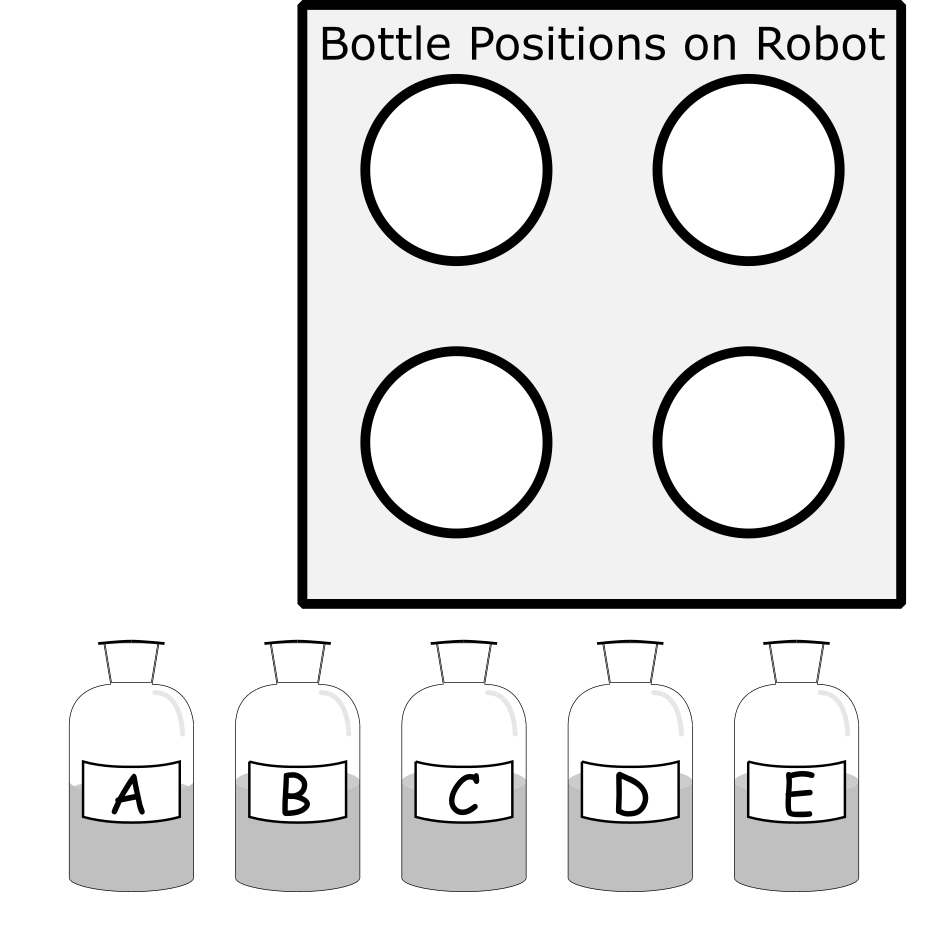
\includegraphics[width=0.3\textwidth]{ch1_Sample_Prep.png}
	}
	\caption{Sample Preperation Robot Problem}
\end{figure}

Whenever a fifth solvent is supposed to be used, the robot has to be stopped and the operator has to manually exchange the bottles of solvents. While this sounds like a typical hard-to-change factor (\textbf{HTC}) there is a major difference: For traditional hard to change factors we try to minimize the number of changes in factor levels. Instead of minimizing the overall number of changes, in this scenario we want to build blocks of experiments in which only a subset of all possible factor levels are used. The problem could be interpreted as generating a blocked design that includes a restriction for each block to use not more than four different solvents.

This paper discusses the problem in more detail. An algorithm to generate optimal designs for this problem is proposed and some resulting designs are evaluated in comparison to completly randomized designs and split-plot designs.

The experienced DoE-expert might skip chapter \ref{splitplots} which gives a short description of split-plot designs and the typical way of analyzing them. Chapter \ref{semisplitplots} describes the sample preperation robot scenario in greater detail. In chapter \ref{algo} we propose an algorithm to generate optimal designs for the described problem. This algorithm is implemented in the rospd-package for the R-software. A short tutorial on how to use the package follows in chapter \ref{rospd}. A comparison of multiple design classes in terms of aliasing and predictive quality is done in chapter \ref{evaluation} before we conclude with a summary and an overview of future work (chapter \ref{summary}).